\documentclass[11pt,a4paper]{article}
\usepackage[margin=1in]{geometry}
\usepackage{kotex}
\usepackage{amsmath,amssymb}
\usepackage{booktabs}
\usepackage{hyperref}
\usepackage{enumitem}
\usepackage{array}
\usepackage{subcaption}
\usepackage{xcolor}
\usepackage{tikz}
\usetikzlibrary{arrows.meta,positioning,calc,fit,shapes.geometric,matrix,backgrounds}

\title{Hands-On Graph Neural Networks Using Python\\Chapter 1--2 상세 정리}
\author{A7610 그래프신경망특론}
\date{\today}

\begin{document}
\maketitle
\tableofcontents
\newpage

\section{Chapter 1: Getting Started with Graph Learning}

\subsection{왜 그래프인가? (Why graphs?)}
그래프는 객체와 객체 사이의 \textbf{관계}를 1급 정보로 다룬다.\
탭ular 데이터는 객체의 속성(attribute)은 잘 담지만, 객체 간 연결 구조를 직접적으로 표현하기 어렵다.

\begin{figure}[h]
\centering
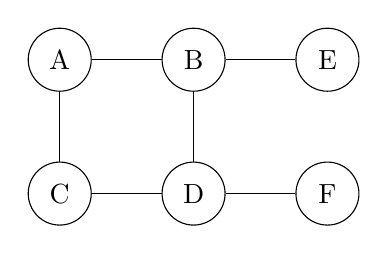
\begin{tikzpicture}[>=Stealth, node distance=1.7cm]
\tikzstyle{n}=[circle,draw,minimum size=8mm]
\node[n] (a) {A};
\node[n, right of=a] (b) {B};
\node[n, below of=a] (c) {C};
\node[n, right of=c] (d) {D};
\node[n, right of=b] (e) {E};
\node[n, right of=d] (f) {F};
\draw (a)--(b);
\draw (a)--(c);
\draw (b)--(d);
\draw (c)--(d);
\draw (b)--(e);
\draw (d)--(f);
\end{tikzpicture}
\caption{관계 구조를 직접 표현하는 그래프 예시}
\end{figure}

\paragraph{그래프가 자연스러운 도메인}
\begin{itemize}[leftmargin=*]
  \item 소셜 네트워크: 사용자(노드)-친구관계(엣지)
  \item 분자 구조: 원자(노드)-결합(엣지)
  \item 교통망: 교차로(노드)-도로(엣지)
  \item 추천 시스템: 사용자/아이템 이분그래프
\end{itemize}

\paragraph{그래프의 장점과 난점}
\begin{itemize}[leftmargin=*]
  \item 장점: 고정 격자(이미지)나 순차(텍스트)로 담기 어려운 \textbf{비정형 관계}를 표현
  \item 난점: 노드 수/연결 수가 샘플마다 다르고 순서 불변성(permutation invariance)을 고려해야 함
\end{itemize}

\begin{figure}[h]
\centering
\begin{tikzpicture}[>=Stealth]
\node[draw,rounded corners,minimum width=3.5cm,minimum height=1cm] (tab) at (0,0) {Tabular data};
\node[draw,rounded corners,minimum width=3.5cm,minimum height=1cm] (graph) at (6,0) {Graph data};
\draw[->,thick] (tab) -- node[above]{관계 정보 추가} (graph);
\node[below=0.2cm of tab] {속성 중심};
\node[below=0.2cm of graph] {속성 + 관계 중심};
\end{tikzpicture}
\caption{테이블 표현에서 그래프 표현으로의 관점 전환}
\end{figure}

\subsection{왜 Graph Learning인가? (Why graph learning?)}
그래프 학습은 그래프 구조와 노드/엣지 특징을 함께 사용해 예측 문제를 푼다.

\subsubsection*{대표 과제}
\begin{enumerate}[leftmargin=*]
  \item Node Classification: 노드 라벨 예측
  \item Link Prediction: 누락/미래 엣지 예측
  \item Graph Classification: 그래프 단위 라벨 예측
  \item Graph Generation: 조건을 만족하는 신규 그래프 생성
\end{enumerate}

\begin{figure}[h]
\centering
\begin{subfigure}{0.48\linewidth}
\centering
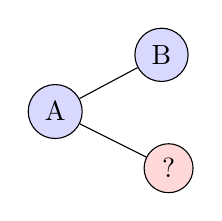
\begin{tikzpicture}[>=Stealth,scale=0.9]
\node[circle,draw,fill=blue!15] (a) at (0,0) {A};
\node[circle,draw,fill=blue!15] (b) at (1.5,0.8) {B};
\node[circle,draw,fill=red!15] (c) at (1.6,-0.8) {?};
\draw (a)--(b);
\draw (a)--(c);
\end{tikzpicture}
\caption{Node classification}
\end{subfigure}
\begin{subfigure}{0.48\linewidth}
\centering
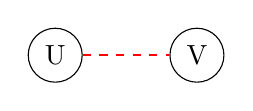
\begin{tikzpicture}[>=Stealth,scale=0.9]
\node[circle,draw] (u) at (0,0) {U};
\node[circle,draw] (v) at (2,0) {V};
\draw[dashed,thick,red] (u)--(v);
\end{tikzpicture}
\caption{Link prediction}
\end{subfigure}

\vspace{0.5em}
\begin{subfigure}{0.48\linewidth}
\centering
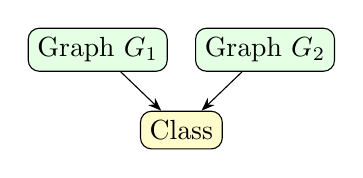
\begin{tikzpicture}[>=Stealth,scale=0.85]
\node[draw,rounded corners,fill=green!10] (g1) at (0,0) {Graph $G_1$};
\node[draw,rounded corners,fill=green!10] (g2) at (2.5,0) {Graph $G_2$};
\node[draw,rounded corners,fill=yellow!20] (cls) at (1.25,-1.2) {Class};
\draw[->] (g1)--(cls);
\draw[->] (g2)--(cls);
\end{tikzpicture}
\caption{Graph classification}
\end{subfigure}
\begin{subfigure}{0.48\linewidth}
\centering
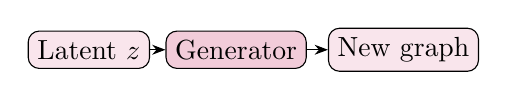
\begin{tikzpicture}[>=Stealth,scale=0.85]
\node[draw,rounded corners,fill=purple!10] (z) at (0,0) {Latent $z$};
\node[draw,rounded corners,fill=purple!20] (gen) at (2.2,0) {Generator};
\node[draw,rounded corners,fill=purple!10] (g) at (4.7,0) {New graph};
\draw[->] (z)--(gen);
\draw[->] (gen)--(g);
\end{tikzpicture}
\caption{Graph generation}
\end{subfigure}
\caption{그래프 학습의 핵심 과제들}
\end{figure}

\subsubsection*{그래프 학습 기법군(책 기준)}
\begin{itemize}[leftmargin=*]
  \item Graph signal processing
  \item Matrix factorization
  \item Random walk
  \item Deep learning (GNN)
\end{itemize}

\subsection{왜 GNN인가? (Why GNN?)}
GNN은 메시지 패싱(message passing)으로 이웃 정보를 반복 집계하여 노드 표현을 업데이트한다.

\[
h_v^{(k)} = \phi^{(k)}\!\left(h_v^{(k-1)},\; \bigoplus_{u\in\mathcal{N}(v)}\psi^{(k)}(h_v^{(k-1)},h_u^{(k-1)},e_{uv})\right)
\]

\noindent 여기서 $\bigoplus$는 합/평균/최대 등 집계 연산이다.

\begin{figure}[h]
\centering
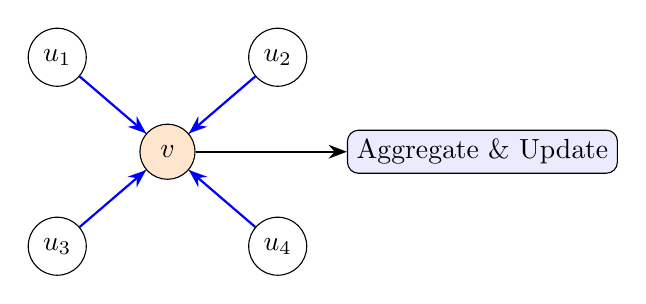
\begin{tikzpicture}[>=Stealth,node distance=1.3cm]
\tikzstyle{n}=[circle,draw,minimum size=7mm]
\node[n,fill=orange!20] (v) at (0,0) {$v$};
\node[n] (n1) at (-1.4,1.2) {$u_1$};
\node[n] (n2) at (1.4,1.2) {$u_2$};
\node[n] (n3) at (-1.4,-1.2) {$u_3$};
\node[n] (n4) at (1.4,-1.2) {$u_4$};
\draw (v)--(n1);
\draw (v)--(n2);
\draw (v)--(n3);
\draw (v)--(n4);
\draw[->,thick,blue] (n1)--(v);
\draw[->,thick,blue] (n2)--(v);
\draw[->,thick,blue] (n3)--(v);
\draw[->,thick,blue] (n4)--(v);
\node[draw,rounded corners,fill=blue!8,minimum width=2.2cm] (agg) at (4,0) {Aggregate \& Update};
\draw[->,thick] (v.east) -- (agg.west);
\end{tikzpicture}
\caption{메시지 패싱: 이웃 정보를 모아 중심 노드 표현을 갱신}
\end{figure}

\paragraph{GNN이 강한 조건}
\begin{itemize}[leftmargin=*]
  \item 문제 복잡도가 높고 관계 구조가 예측 성능에 큰 영향을 줄 때
  \item 대규모 데이터에서 표현학습(representation learning)이 필요할 때
\end{itemize}

\paragraph{주의점}
\begin{itemize}[leftmargin=*]
  \item 과도한 레이어 깊이는 over-smoothing을 유발할 수 있음
  \item 소규모 데이터/단순 규칙 문제에서는 비딥러닝 기법이 효율적일 수 있음
\end{itemize}

\newpage
\section{Chapter 2: Graph Theory for Graph Neural Networks}

\subsection{그래프의 기본 성질}
그래프는 보통 $G=(V,E)$로 표기한다. $V$는 노드 집합, $E$는 엣지 집합이다.

\begin{figure}[h]
\centering
\begin{subfigure}{0.48\linewidth}
\centering
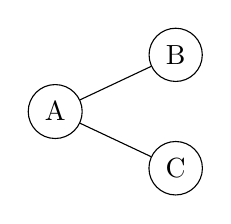
\begin{tikzpicture}[>=Stealth,scale=0.9]
\node[circle,draw] (a) at (0,0) {A};
\node[circle,draw] (b) at (1.7,0.8) {B};
\node[circle,draw] (c) at (1.7,-0.8) {C};
\draw (a)--(b);
\draw (a)--(c);
\end{tikzpicture}
\caption{Undirected graph}
\end{subfigure}
\begin{subfigure}{0.48\linewidth}
\centering
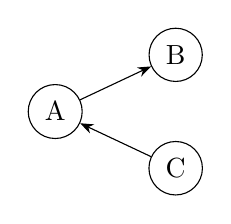
\begin{tikzpicture}[>=Stealth,scale=0.9]
\node[circle,draw] (a) at (0,0) {A};
\node[circle,draw] (b) at (1.7,0.8) {B};
\node[circle,draw] (c) at (1.7,-0.8) {C};
\draw[->] (a)--(b);
\draw[->] (c)--(a);
\end{tikzpicture}
\caption{Directed graph}
\end{subfigure}
\caption{방향성 여부}
\end{figure}

\begin{figure}[h]
\centering
\begin{subfigure}{0.48\linewidth}
\centering
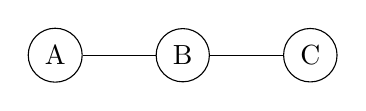
\begin{tikzpicture}[>=Stealth,scale=0.9]
\node[circle,draw] (a) at (0,0) {A};
\node[circle,draw] (b) at (1.8,0) {B};
\node[circle,draw] (c) at (3.6,0) {C};
\draw (a)--(b);
\draw (b)--(c);
\end{tikzpicture}
\caption{Unweighted}
\end{subfigure}
\begin{subfigure}{0.48\linewidth}
\centering
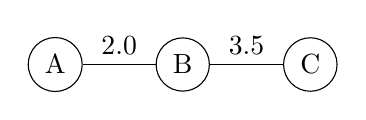
\begin{tikzpicture}[>=Stealth,scale=0.9]
\node[circle,draw] (a) at (0,0) {A};
\node[circle,draw] (b) at (1.8,0) {B};
\node[circle,draw] (c) at (3.6,0) {C};
\draw (a)-- node[above]{2.0} (b);
\draw (b)-- node[above]{3.5} (c);
\end{tikzpicture}
\caption{Weighted}
\end{subfigure}
\caption{가중치 여부}
\end{figure}

\begin{figure}[h]
\centering
\begin{subfigure}{0.48\linewidth}
\centering
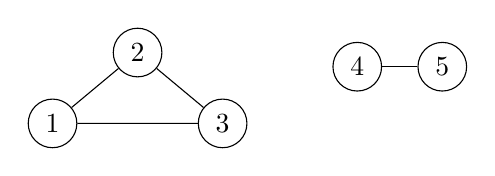
\begin{tikzpicture}[scale=0.9]
\node[circle,draw] (a) at (0,0) {1};
\node[circle,draw] (b) at (1.2,1) {2};
\node[circle,draw] (c) at (2.4,0) {3};
\node[circle,draw] (d) at (4.3,0.8) {4};
\node[circle,draw] (e) at (5.5,0.8) {5};
\draw (a)--(b)--(c)--(a);
\draw (d)--(e);
\end{tikzpicture}
\caption{Disconnected}
\end{subfigure}
\begin{subfigure}{0.48\linewidth}
\centering
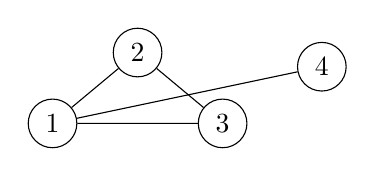
\begin{tikzpicture}[scale=0.9]
\node[circle,draw] (a) at (0,0) {1};
\node[circle,draw] (b) at (1.2,1) {2};
\node[circle,draw] (c) at (2.4,0) {3};
\node[circle,draw] (d) at (3.8,0.8) {4};
\draw (a)--(b)--(c)--(a);
\draw (a)--(d);
\end{tikzpicture}
\caption{Connected}
\end{subfigure}
\caption{연결성 여부}
\end{figure}

\subsection{중요 그래프 유형}
\begin{figure}[h]
\centering
\begin{tikzpicture}[scale=0.9]
\node[draw,rounded corners,fill=green!10,minimum width=2.6cm] (t) at (0,0.8) {Tree};
\node[draw,rounded corners,fill=green!10,minimum width=2.6cm] (rt) at (3.5,0.8) {Rooted Tree};
\node[draw,rounded corners,fill=green!10,minimum width=2.6cm] (dag) at (7,0.8) {DAG};
\node[draw,rounded corners,fill=green!10,minimum width=2.6cm] (bi) at (1.75,-1.0) {Bipartite};
\node[draw,rounded corners,fill=green!10,minimum width=2.6cm] (k) at (5.25,-1.0) {Complete};
\draw[->] (t)-- node[left]{무사이클} (bi);
\draw[->] (rt)-- node[right]{루트 지정} (dag);
\draw[->] (dag)--(k);
\end{tikzpicture}
\caption{자주 등장하는 그래프 유형 개요}
\end{figure}

\subsection{기초 객체: degree, neighbors, path}
\begin{itemize}[leftmargin=*]
  \item 무방향 degree: $\deg(v)$
  \item 유방향 indegree/outdegree: $\deg^-(v),\deg^+(v)$
  \item path: 엣지들의 연쇄, cycle: 시작과 끝이 같은 path
\end{itemize}

\begin{figure}[h]
\centering
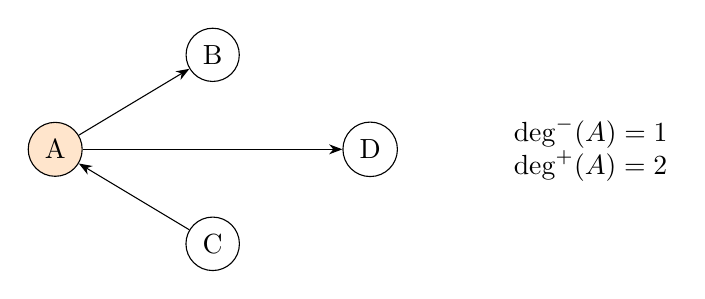
\begin{tikzpicture}[>=Stealth]
\node[circle,draw,fill=orange!20] (a) at (0,0) {A};
\node[circle,draw] (b) at (2,1.2) {B};
\node[circle,draw] (c) at (2,-1.2) {C};
\node[circle,draw] (d) at (4,0) {D};
\draw[->] (a)--(b);
\draw[->] (c)--(a);
\draw[->] (a)--(d);
\node[align=left] at (6.8,0) {$\deg^-(A)=1$\\$\deg^+(A)=2$};
\end{tikzpicture}
\caption{유방향 그래프에서의 indegree/outdegree 예시}
\end{figure}

\subsection{그래프 측도: Centrality와 Density}
\subsubsection*{Centrality}
\begin{itemize}[leftmargin=*]
  \item Degree centrality: 연결 수 기반 중요도
  \item Closeness centrality: 다른 노드까지 평균 최단거리 기반 접근성
  \item Betweenness centrality: 최단경로 사이의 중개자 역할
\end{itemize}

\begin{figure}[h]
\centering
\begin{tikzpicture}[scale=1.0]
\node[circle,draw,fill=red!35,minimum size=10mm] (a) at (0,0) {A};
\node[circle,draw,fill=orange!30,minimum size=9mm] (b) at (1.6,1.1) {B};
\node[circle,draw,fill=orange!30,minimum size=9mm] (c) at (1.6,-1.1) {C};
\node[circle,draw,fill=yellow!25,minimum size=8mm] (d) at (3.2,1.1) {D};
\node[circle,draw,fill=yellow!25,minimum size=8mm] (e) at (3.2,-1.1) {E};
\draw (a)--(b)--(d);
\draw (a)--(c)--(e);
\draw (b)--(c);
\node[right] at (4.6,0) {색/크기 = 상대적 centrality};
\end{tikzpicture}
\caption{중심성 직관: 중심부 노드가 정보 흐름에 더 큰 영향}
\end{figure}

\subsubsection*{Density}
\[
\rho_{\text{undir}}=\frac{|E|}{|V|(|V|-1)/2}, \qquad
\rho_{\text{dir}}=\frac{|E|}{|V|(|V|-1)}
\]
밀도는 연결의 조밀함을 나타내며, 일반적으로 낮으면 희소(sparse), 높으면 조밀(dense) 그래프로 본다.

\subsection{그래프 표현 방법}

\begin{figure}[h]
\centering
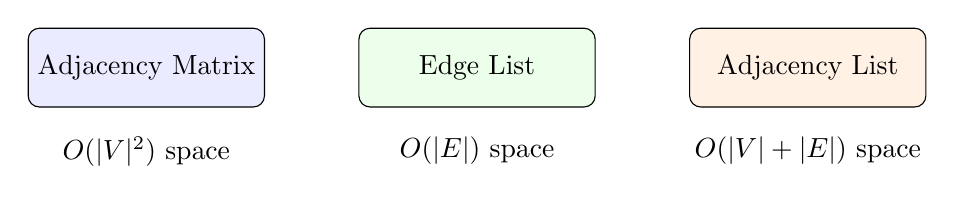
\begin{tikzpicture}[>=Stealth]
\node[draw,rounded corners,fill=blue!8,minimum width=3.0cm,minimum height=1cm] (am) at (0,0) {Adjacency Matrix};
\node[draw,rounded corners,fill=green!8,minimum width=3.0cm,minimum height=1cm] (el) at (4.2,0) {Edge List};
\node[draw,rounded corners,fill=orange!10,minimum width=3.0cm,minimum height=1cm] (al) at (8.4,0) {Adjacency List};
\node[below=0.25cm of am] {$O(|V|^2)$ space};
\node[below=0.25cm of el] {$O(|E|)$ space};
\node[below=0.25cm of al] {$O(|V|+|E|)$ space};
\end{tikzpicture}
\caption{세 가지 대표 그래프 저장 방식}
\end{figure}

\begin{table}[h]
\centering
\begin{tabular}{@{}>{\raggedright\arraybackslash}p{3.2cm}p{5.6cm}p{5.6cm}@{}}
\toprule
표현 방식 & 장점 & 단점 \\ \midrule
Adjacency Matrix & 엣지 존재 여부 확인이 $O(1)$, 행렬 연산 활용 용이 & 공간복잡도 $O(|V|^2)$로 대규모 희소 그래프에서 비효율 \\
Edge List & 저장이 단순, 희소 그래프 저장 효율 높음 & 엣지 조회 시 리스트 탐색이 필요해 느릴 수 있음 \\
Adjacency List & 공간복잡도 $O(|V|+|E|)$, 이웃 순회 효율적 & 엣지 존재 확인은 평균적으로 Matrix보다 느림 \\
\bottomrule
\end{tabular}
\caption{그래프 표현 방식 트레이드오프}
\end{table}

\subsection{그래프 탐색 알고리즘: BFS와 DFS}

\subsubsection*{BFS (Breadth-First Search)}
\begin{itemize}[leftmargin=*]
  \item 큐를 이용해 레벨 순서로 탐색
  \item 무가중치 그래프 최단거리 탐색에 유리
  \item 시간복잡도: $O(|V|+|E|)$
\end{itemize}

\begin{figure}[h]
\centering
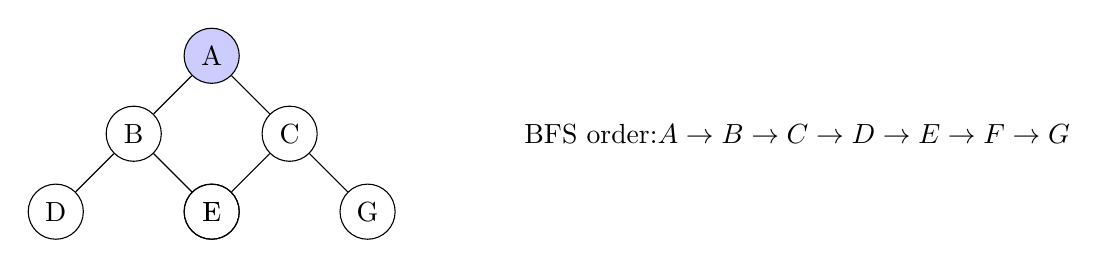
\begin{tikzpicture}[>=Stealth, node distance=1.4cm]
\tikzstyle{n}=[circle,draw,minimum size=7mm]
\node[n,fill=blue!20] (a) {A};
\node[n,below left of=a] (b) {B};
\node[n,below right of=a] (c) {C};
\node[n,below left of=b] (d) {D};
\node[n,below right of=b] (e) {E};
\node[n,below left of=c] (f) {F};
\node[n,below right of=c] (g) {G};
\draw (a)--(b) (a)--(c) (b)--(d) (b)--(e) (c)--(f) (c)--(g);
\node[right=2.5cm of c,align=left] {BFS order:$A\rightarrow B\rightarrow C\rightarrow D\rightarrow E\rightarrow F\rightarrow G$};
\end{tikzpicture}
\caption{BFS: 레벨 단위 확장}
\end{figure}

\subsubsection*{DFS (Depth-First Search)}
\begin{itemize}[leftmargin=*]
  \item 스택/재귀로 한 경로를 깊게 탐색 후 백트래킹
  \item 사이클 탐지, 위상정렬, connected component 탐색 기반
  \item 시간복잡도: $O(|V|+|E|)$
\end{itemize}

\begin{figure}[h]
\centering
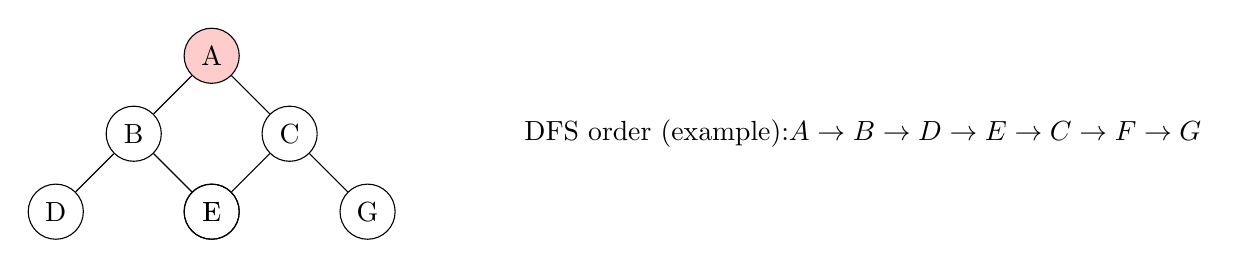
\begin{tikzpicture}[>=Stealth, node distance=1.4cm]
\tikzstyle{n}=[circle,draw,minimum size=7mm]
\node[n,fill=red!20] (a) {A};
\node[n,below left of=a] (b) {B};
\node[n,below right of=a] (c) {C};
\node[n,below left of=b] (d) {D};
\node[n,below right of=b] (e) {E};
\node[n,below left of=c] (f) {F};
\node[n,below right of=c] (g) {G};
\draw (a)--(b) (a)--(c) (b)--(d) (b)--(e) (c)--(f) (c)--(g);
\node[right=2.5cm of c,align=left] {DFS order (example):$A\rightarrow B\rightarrow D\rightarrow E\rightarrow C\rightarrow F\rightarrow G$};
\end{tikzpicture}
\caption{DFS: 깊이 우선 탐색 후 백트래킹}
\end{figure}

\subsection{BFS vs DFS 요약 비교}
\begin{table}[h]
\centering
\begin{tabular}{@{}lll@{}}
\toprule
항목 & BFS & DFS \\ \midrule
핵심 자료구조 & Queue & Stack / Recursion \\
탐색 특징 & 가까운 노드부터 확장 & 한 분기를 깊게 탐색 \\
강점 & 무가중치 최단경로 & 구조 탐색/사이클 관련 문제 \\
약점 & 넓은 그래프에서 메모리 부담 & 최단경로 보장 안 됨 \\
\bottomrule
\end{tabular}
\caption{두 탐색 알고리즘의 실전 선택 기준}
\end{table}

\newpage
\section{시험/발표 포인트 정리}
\begin{enumerate}[leftmargin=*]
  \item ``왜 그래프인가''를 \textbf{속성+관계 정보 결합} 관점에서 설명할 것
  \item 그래프 학습 4대 과제(Node/Link/Graph/Generation)를 사례와 함께 구분할 것
  \item GNN의 핵심이 \textbf{이웃 집계(message passing)}임을 수식과 직관으로 설명할 것
  \item 방향성/가중치/연결성과 특수 그래프(Tree, DAG, Bipartite)를 명확히 구분할 것
  \item 중앙성/밀도/표현방식(Matrix/List)의 트레이드오프를 비교할 것
  \item BFS/DFS의 선택 기준을 문제 유형(최단거리 vs 구조탐색)에 연결할 것
\end{enumerate}

\end{document}

